\section{Data understanding and preparation}
We focused our work on the matches dataset that contains tennis matches played in many tournaments across the world over the last five years, it includes both male and female players and has 186.129 records and 49 features. We decided not to do any cleaning or integration on the male and female datasets since they were only used to get the sex for each player.

\subsection{Data understanding}
The data understanding task focuses on analyzing the dataset and its integration by removing duplicated values, fixing missing values and solving the possible outliers.
\subsubsection{Data semantics}
In this phase we focused on understanding the meaning of each feature inside the dataset.
\begin{itemize}
    \item \textbf{tourney\_id}: it's a \textbf{string} that uniquely identifies each tournament. It is mainly composed by two part separated by a dash "-", where the first one indicates the year when the tournament was played and the second one refers to the tournament identifier, i.e. '2018-W-WITF-EGY-03A-2018'. The dataset contains some null value for this feature (only for the last tournament), while it has 4853 unique values.
    \item \textbf{tourney\_name}: it's a string that represent the name of the tournament and it's not unique because the name of the tournament is usually the same over the years. It has some missing values only in the last part of the dataset.
    \item \textbf{surface}: it indicates the surface where the matches took place. It's a categorical attribute which its possible values are: hard, clay, grass and carpet. Only few matches are missing this feature.
    \item \textbf{draw\_size}: it's a float that indicates the number of players in a tournament.
    \item \textbf{tourney\_level}: it's a string indicates whether the tournament is for male or female players and also its level (mastr, ATP500, ATP1000 etc.). Has some missing values in the last part of the dataset just like for the tourney\_id.
    \item \textbf{tourney\_date}: it's the date when the match took place. In the dataset it's a float in the form YYYYMMDD. To use it as real date, a parsing to a date type is needed. Missing values are present only in the last part of the dataset.
    \item \textbf{match\_number}: it's a float number that represents the match number in a tournament. Due to its meaning, it should be parsed to an integer.
    \item \textbf{winner\_id}: in the dataset, it's a float representing the id of the match winner. For sure, it is unique for the player with the same gender, while the same id can appear for a male player and for a female player as well, since they play in different tours (ATP and WTA).
    \item \textbf{winner\_entry}: it's a string that indicates how a player joined the tournament. There are a lot of missing values for this feature.
    \item \textbf{winner\_hand}: it's a string representing the winner player's favourite hand. Its possible values are 'U' for unknown, 'R' for right and 'L' for left. Actually there are also null values, but they can be treated as unknown.
    \item \textbf{winner\_ht and loser\_ht}: float representing the winner player's height. There are a lot of missing values for this field that can not be inferred by other records where this it's filled.
    \item \textbf{winner\_ioc and loser\_ioc}: a 3-character string representing the player's nationality. Some of them have been written using different standards. For instance, a German player is present both as 'GER' and as 'DEU'. Also, some players appears with more than one nationality because they switched nationality during the last years.
    \item \textbf{winner\_age and loser\_age}: a float that indicates the age of the winner. The decimal part represents the percentage of the days days left to birthday. Some of these values are missing in the dataset, but few of them can be precisely inferred.
    \item \textbf{best\_of}: a float indicating the number of set for a match. We parse it to an integer.
    \item \textbf{round}: the match round (e.g. F stands for final and SF for semifinal).
    \item \textbf{minutes}: indicates how much a match lasted. It's a float that we converted to an integer.
    \item \textbf{w\_ace and l\_ace}: number of aces (valid serve won, first or second, not touched by the opposing player). It's a float, but actually is an integer.
    \item \textbf{w\_df and l\_df}: number of double faults committed by the player (more specifically the number of invalid second serves). It's a float converted to int.
    \item \textbf{w\_svpt and l\_svpt}: this may be confusing, it isn't the number of points obtained after a player serve but the number of serves done by the player (the former is referred on specialised sites as serve points won).
    \item \textbf{w\_1stIn and l\_2stIn}: number of valid first serve by the player.
    \item \textbf{w\_1stWon and l\_1stWon}: number of points won after a valid first serve by the player.
    \item \textbf{w\_2ndWon and l\_2ndWon}: number of points won after a valid second serve by the player, be aware that a point lost after a second serve could be a double fault (this means that the second serve wasn't valid).
    \item \textbf{w\_SvGms and l\_SvGms}: number of games (not points) where the player was serving.
    \item \textbf{w\_bpSaved and l\_bpSaved}: number of breakpoints (the player is a point from losing a game where he's serving) saved (the player serving won the point).
    \item \textbf{w\_bpFaced and l\_bpFaced}: number of breakpoints that the player faced (see previous feature).
    \item \textbf{w\_rank and l\_rank}: the player's rank, in tennis points are awarded based on the performance at each tournament.
    \item \textbf{w\_rank\_points and l\_rank\_points}: the player's ranking points.
    \item \textbf{tourney\_revenue}: the tourney revenue coming from ticket sales etc. It isn't the prize of the tournament (which would have been more interesting for a player analysis).
    \item \textbf{tourney\_spectators}: number of spectators of the entire tournament.
\end{itemize}

\subsubsection{Type casting}
In this dataset, most of the features have an incorrect data type. We parse the tourney\_date from float to pandas date type. Furthermore, every float attribute has been parsed to integer except for the winner/loser age and the tourney\_revenue.

\subsubsection{Dropping useless matches}
There are many matches without any statistics, highlighted in \autoref{fig:features_heatmap}. Such matches are from minor tournaments and the players who played in them don't have many  matches in the dataset, we decided to drop them.
\begin{figure}[H]
    \centering
    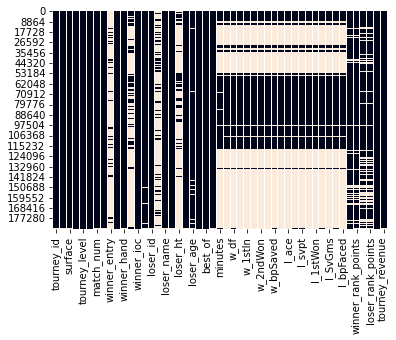
\includegraphics[width= 0.55\linewidth]{images/data_understanding/features_heatmap.png}
    \caption{The missing values heatmap.}
    \label{fig:features_heatmap}
\end{figure}
Furthermore, starting from line n. 186073 to the end, we found a block of records that is a copy of some matches of the Taipei tournament, but with some field left empty. Having noticed this, we dropped this useless part of the dataset.

\subsubsection{Dropping useless features:}
For our purpose, an analysis of the players, some features are not interesting or straight useless, so we decided to drop them. We don't need the \textbf{tourney name}, since we don't differentiate between the tournaments (masters atp, ATP1000 etc.), moreover we already have the \textbf{tourney id} and \textbf{date}.

The \textbf{draw size} is useless for the players and the \textbf{tourney level} can't be used to differentiate between men and women, since the latter can play the same kind of tournaments of the former. For what concerns \textbf{match num}, it's a progressive number for the matches of a tournament, sometimes is totally arbitrary, we don't need it.

\textbf{Winner entry} (and \textbf{loser entry}) is a string that shows if the player qualified by a wildcard, as a lucky loser etc., it's not a very useful attribute since no site lists them, moreover is the feature with the most missing values.

The last features we dropped are \textbf{tourney revenue} and \textbf{tourney spectators}, the former is the amount of revenue generated by the tournament and not the winner prize which would have been really interesting. The latter is the amount of spectators of the entire tournament, not match to match, so we can't retrieve information about how famous the players involved in a certain match are or if they can play better under more pressure.

\subsubsection{Dropping duplicates}
We found that the matches dataset has 302 duplicated records. Due to the domain of this dataset, these duplicates are useless, so we drop them.

\subsubsection{Data integration}
The data integration task consists in solving the various issues found in the dataset by filling the missing values, where it's possible, and fixing the various problems that may arise (e.g.: players with two hands preferred or with more than one ioc).
\paragraph{Player id and name}
In our analysis, we found that there are three players ('Guy Stokman', 'Giuseppe Tresca', 'Kuan Yi Lee') that appear in the dataset with more than one id associated. Moreover, there's only one player with an actual homonym (Kuan Yi Lee), one is a male (id: 134120) and the other one is female (id: 221745), but we discovered that the actual name of the male player is Kuan-Yi, so we change his name to differentiate between the two players. For what concerns the other two players, we assign them their last id.

Deepening the analysis, we found that ids are shared only between a male and female player and this is allowed since different tours exist (ATP and WTA) for each sex, so we don't need to apply any change, moreover we won't work with ids so this won't affect our analysis.

\paragraph{Surface}
We found that the "surface" feature has some null values. Moreover, the number of tournaments without a surface are 42 while the number of matches without a surface are 117. In order to solve this problem, for those tournaments that lack the surface  we can retrieve it if at least one match of the same tournament has it. Unluckily there are no tournaments for which we can retrieve the surface (all of them are from the Davis or Federation cup, where the surface changes from event to event), so we chose to sample such values from the distribution of the surfaces.

\paragraph{Winner/loser hand}
We have to manage the missing values for both "winner\_hand" and "loser\_hand". To do this, we checked if the value is missing only for a particular player or if he/she never has the hand defined and, in this case, we assign it to him/her. After this step, however, the missing values are still present, but since the domain of this feature is {'U', 'L', 'R'}, we can safely treat null values as 'U'. The players with unknown hand are 1840. Among them, we retrieved the actual preferred hand for one player, Amina Anshba who is left-handed.

\paragraph{Winner/loser height}
This feature contains missing values too, so we address this problem as before, looking for those players that have a known height somewhere in the dataset. A deeper analysis show us that 'David Goffin' has two heights registered: 180 cm and 163 cm. Since his real height is the first one, we fixed it in in all occurrences in which he appears.

\paragraph{Winner/loser ioc}
Since there are no missing values for this feature, we only need to check if there are players with more than one ioc. Since we dropped records and players that have played too few matches, we haven't found players with more than one ioc. In the original dataset instead, it happens. Anyway, we found that player called 'Xinmu Zhou', has 'UNK' nationality, but he is Chinese actually, so we assign him 'CHN'. Lastly, we discovered that sometimes, the acronyms of the nations are wrong, since some of them don't follow the international standard (e.g.: GRE for Greece instead of GRC, or TPE for Taiwan instead of TWN) or have both at the same time (e.g.: DEU and GER for Germany), so we fixed them, at least the ones we found.

\paragraph{Winner/loser age}
There are 58 players with unknown age. Among them there are only two players whose age can be inferred from the other information inside the dataset, we fix the missing ages during the data preparation task. 

\paragraph{Winner/loser rank} This information is missing for those players that played only few matches. We fixed the missing values with the last tournament rank for each player (or the next if not present) that already had a rank. For those without rank we assumed they didn't have any points so we assigned them the maximum rank in found in the dataset.

\paragraph{Winner/loser rank points} Same work as for the rank feature, instead this time we assign the minimum value for those players without any rank points (they are the same we found during the rank integration).

\subsubsection{Outlier detection}
Given that all the feature distribution are Gaussian or half normal, to analyze outliers we must first compute the first quartile, the third quartile, the median and the interquartile for each feature. Then we compute the lower bound $L=Q1 - 1.5 * IQR$ and the upper bound $U=Q1 + 1.5 * IQR$ for each feature. In case some numerical data was less or greater than the lower or upper bound respectively, we can identify an outlier. For half-normal distribution we don't consider the lower bound. In case of an outlier that can be fixed with a real value, we do it. In this way we found, for example, two players that have too low height and, in fact, these data were wrong. We fixed it with the players' real height. Whereas high values correspond to those players that are actually tall. We have applied this analysis for every numerical feature.
\begin{figure}[H]
    \centering
    \subfloat[Before detection]{{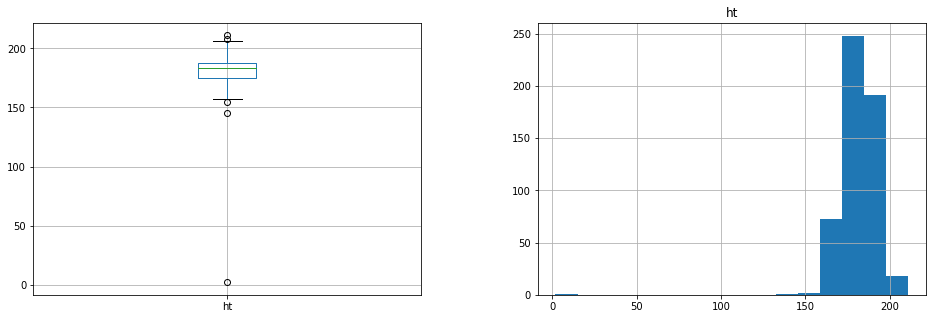
\includegraphics[width= 0.5\linewidth]{images/data_understanding/ht_before_detection.png}}}%
    \subfloat[After detection]{{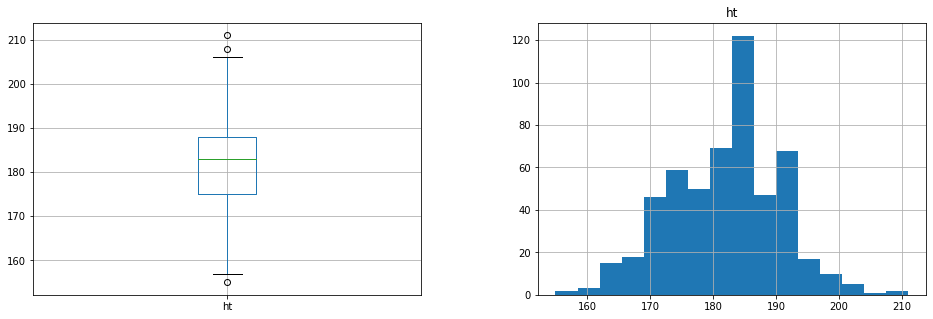
\includegraphics[width= 0.5\linewidth]{images/data_understanding/ht_after_detection.png}}}%
    \caption{An example of a feature's distribution after dealing with outliers.}
    \label{fig:before_and_after_detection}
\end{figure}

\subsubsection{Correlations}
We plot the correlation matrix in order to visualize whether there are correlation between the features. In \autoref{fig:corr_matrix_tennis_matches}, the more the color is red the more the features are correlated.
\begin{figure}[H]
    \centering
    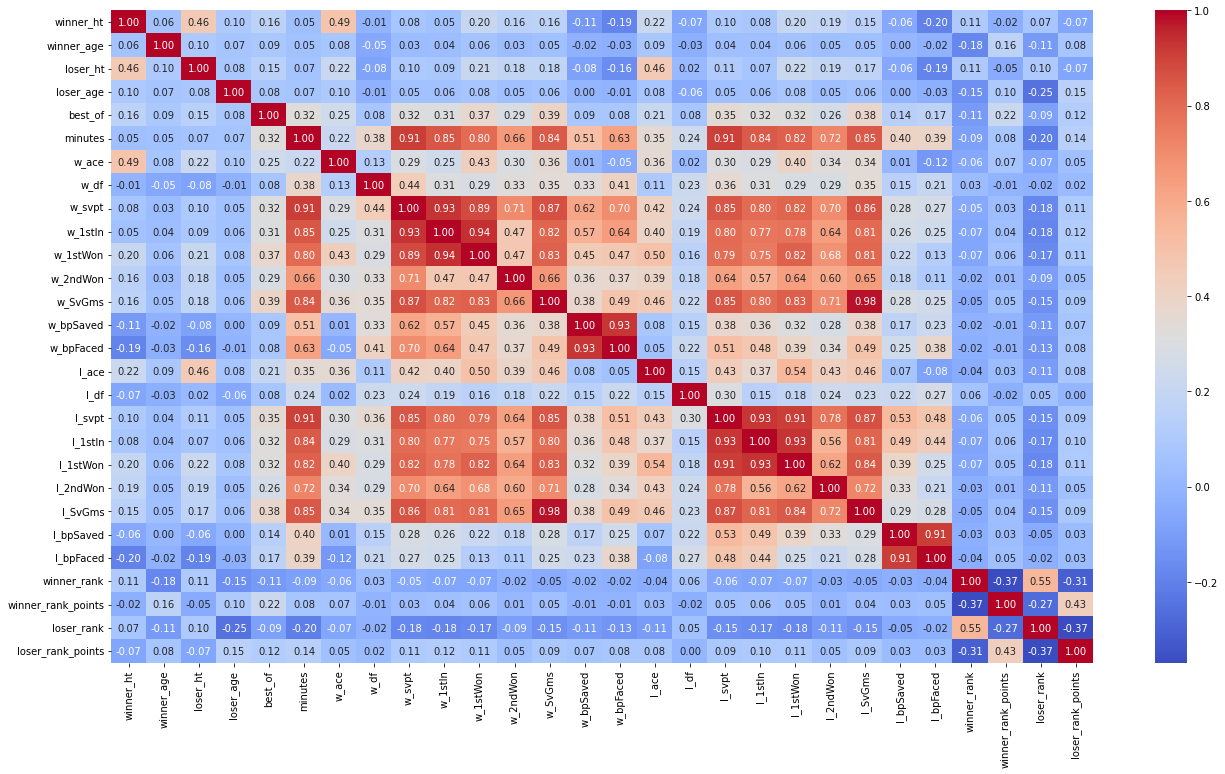
\includegraphics[width= 0.74\linewidth]{images/data_understanding/correlation.png}
    \caption{Correlation matrix of the tennis matches dataset.}
    \label{fig:corr_matrix_tennis_matches}
\end{figure}
After looking at the correlation matrix we dropped the minutes feature since we deemed it as useless after doing a huge help during the outlier detection by showing "inusual matches". 